\documentclass[t,11pt]{beamer}

\usepackage[francais]{babel}
\usepackage[T1]{fontenc}
\usepackage[utf8]{inputenc}
\usepackage{hyperref}

\usetheme{Warsaw}
\setbeamercolor{background canvas}{bg=yellow!10!white}


\title{Introduction pragmatique à Git}
\author{K\'evin Unger\hspace{1mm} \newline kevin.unger@fresnel.fr}
\institute
{
        Institut Fresnel\\
        \url{https://github.com/kevung/git-presentation.git}
}
\date{\today}

\begin{document}

%----------------------------------------------
\begin{frame}[plain,c]
        \titlepage
\end{frame}

%----------------------------------------------
%table des matieres
\begin{frame}[c]
        \frametitle{Sommaire}
        \tableofcontents[hideallsubsections]
\end{frame}

%----------------------------------------------
%table des matieres auto a chaque section
\AtBeginSection[]{
\begin{frame}[c]
        \tableofcontents[currentsection,hideallsubsections]
\end{frame}
}

%----------------------------------------------
\section{Git?! A quoi ça sert\ldots}


\subsection{Situation n. 1}
\begin{frame}[label=sit1]
        \frametitle{Situation n. 1}
        \framesubtitle{Comment garder des traces sans perdre la tête?}
        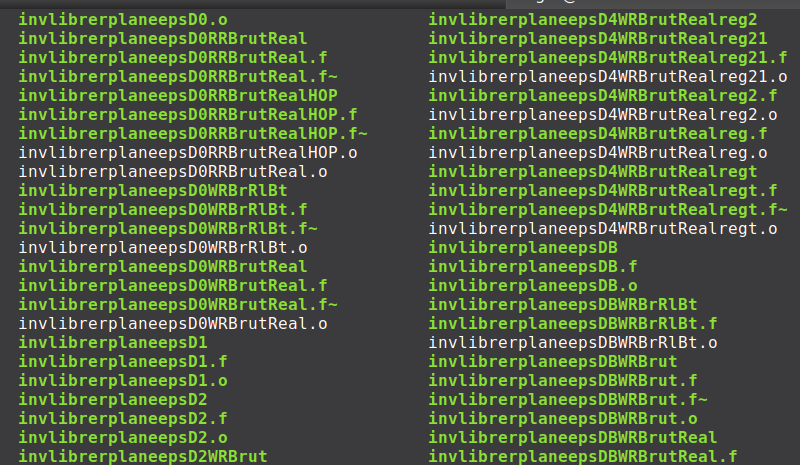
\includegraphics[width=\linewidth]{./img/bazar_crop2}
\end{frame}


\subsection{Situation n. 2}
\begin{frame}[label=sit2]
        \frametitle{Situation n. 2}
        \framesubtitle{Comment tester sans avoir peur de tout casser?}
\end{frame}


\subsection{Situation n. 3}
\begin{frame}[label=sit3]
        \frametitle{Situation n. 3}
        \framesubtitle{Comment travailler simultane\'ment sur un même document?}
\end{frame}

%----------------------------------------------
\section{Garder des traces proprement}

\subsection{Principe}
\begin{frame}[c]
        \frametitle{Principe}
        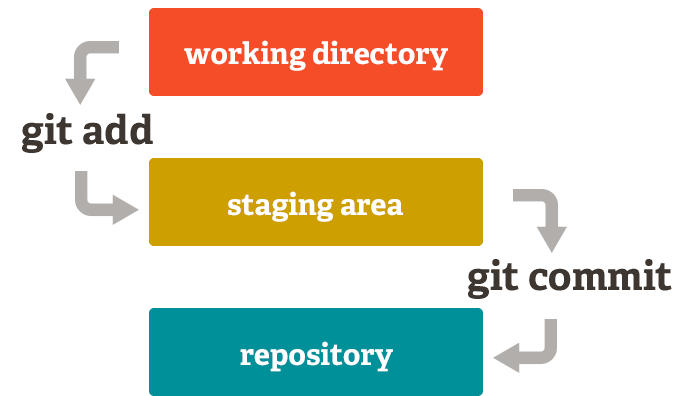
\includegraphics[width=\linewidth]{./img/git_staging_area}
        \newline
        \hspace*{15pt}
        \href{https://git-scm.com/about/staging-area}{{\tiny (source: Pro Git)}}
\end{frame}

\subsection{Cycle de vie d'un fichier}
\begin{frame}[c]
        \frametitle{Cycle de vie d'un fichier}
        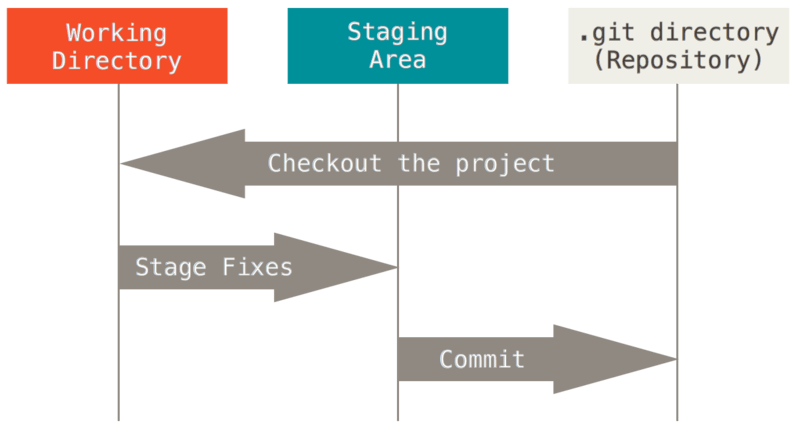
\includegraphics[width=\linewidth]{./img/git_cycle}
        \newline
        \hspace*{15pt}
        \href{https://git-scm.com/book/fr/v2/Les-bases-de-Git-Enregistrer-des-modifications-dans-le-d\%C3\%A9p\%C3\%B4t}{{\tiny (source: Pro Git)}}
\end{frame}


\subsection{Exemple d'historique}
\begin{frame}[c]
        \frametitle{Exemple d'historique}
        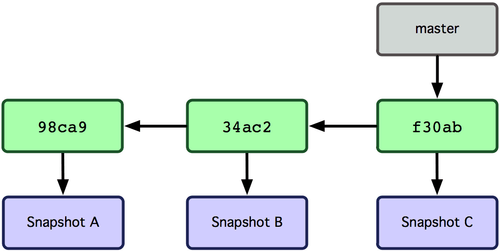
\includegraphics[width=\linewidth]{./img/master_branch}
        \newline
        \hspace*{15pt}
        \href{https://git-scm.com/book/fr/v1/Les-branches-avec-Git-Ce-qu-est-une-branche}{{\tiny (source: Pro Git)}}
\end{frame}

\subsection{Cinq commandes}
\begin{frame}[t]
        \frametitle{Cinq commandes}
        \begin{columns}
                \column{0.5\linewidth}
                \begin{block}{Affiche l'\'etat du d\'ep\^ot}
                        \centering
                        git status
                \end{block}
        \end{columns}

        \begin{columns}
                \column{0.5\linewidth}
                \begin{block}{Ajoute pour le prochain archivage}
                        \centering
                        git add
                \end{block}
                \column{0.5\linewidth}

                \begin{block}{Archive}
                        \centering
                        git commit
                \end{block}
        \end{columns}

        \begin{columns}
                \column{0.5\linewidth}
                \begin{block}{Affiche l'historique}
                        \centering
                        git log
                \end{block}

                \column{0.5\linewidth}
                \begin{block}{Restaure l'\'etat d'une archive}
                        \centering
                        git checkout \emph{mon-commit}
                \end{block}
        \end{columns}
\end{frame}

%----------------------------------------------
\section{Exp\'erimenter en toute s\'ecurit\'e}

\subsection{Principe}
\begin{frame}
        \frametitle{Principe}
        Principe du branching
\end{frame}

%----------------------------------------------
\section{Travailler \`a plusieurs (simultan\'ement) }

\subsection{Principe}
\begin{frame}
        \frametitle{Principe}
        Principe d'un d\'ep\^ot
\end{frame}

%-----------------------------------------------
\appendix
\begin{frame}[c]
        \frametitle{Annexes}
        \tableofcontents[hideallsubsections]
\end{frame}

%-----------------------------------------------
\section{Configurer Git}
\subsection{Configuration initiale}
\begin{frame}
        \frametitle{Configuration initiale}
        \begin{block}{Identit\'e}
                git config --global user.name "Augustin Fresnel"
        \end{block}
        
        \begin{block}{Email}
                git config --global user.email "augustin.fresnel@fresnel.fr"
        \end{block}

        \begin{block}{Editeur}
                git config --global core.editor emacs
        \end{block}
\end{frame}

\subsection{Les alias}
\begin{frame}
        \frametitle{Les alias}
        \begin{itemize}
                \item status
                \item commit
                \item checkout
                \item branch
        \end{itemize}
\end{frame}

%-----------------------------------------------
\section{Explorer l'historique}
\subsection{git difftool}
\begin{frame}
        \frametitle{git difftool}
        kdiff3, image
\end{frame}

\subsection{Interfaces Git graphiques}
\begin{frame}
        \frametitle{Interfaces Git graphiques}
\end{frame}


%-----------------------------------------------
\section{G\'erer les conflits de fusion}
\subsection{git mergetool}
\begin{frame}
        \frametitle{git mergetool}
        screenshot avec reglement fusion
        sans et avec kdiff3
\end{frame}

\section{Travailler sur plusieurs branches}
\subsection{git stash}
\begin{frame}
        \frametitle{git stash}
\end{frame}

\subsection{git cherry-pick}
\begin{frame}
        \frametitle{git cherry-pick}
\end{frame}

%-----------------------------------------------
\section{Int\'egration avec le shell}
\begin{frame}
        \frametitle{Int\'egration avec le shell}
        zsh + oh-my-zsh + plugin git
\end{frame}
\end{document}
